\section{Subsistema: Perfuração e Coleta}

  \subsection{Sistema de Perfuração}
  
  Para o sistema de perfuração algumas pesquisas e discussões foram feitas para escolher um sistema que pudesse ser realizado. Foram defiidas duas opções possíveis para serem comparadas e analisadas e depois decidir a que se encaixa melhor nos requisitos do projeto.

  \textbf{Opção A}: Usar uma broca para perfurar o plástico e a terra, ao completar este
  processo, um dispositivo é acionado para realizar a troca da peça broca para
  a peça sensor, o sensor de umidade é então estendido até o solo do buraco e
  coleta os dados solicitados. Após a coleta dos dados o sensor é recolhido e o
  carrinho segue em frente para mais uma perfuração.

  \textbf{Opção B}: Usar um tubo puntiforme contendo o sensor, havendo na ponta do tubo
  aberturas levemente maiores que as dimensões dos terminais do sensor. O tubo
  terá um motor para empurrá-lo até a lona e fazer o furo desejado; um servo
  motor estenderá o sensor para que ele possa fazer a medição da umidade.

  O grupo optou pela opção B pelos seguintes fatores:

  \begin{itemize}
    \item Dificuldade em elaborar um mecanismo para alternar a broca e o sensor
    conforme descrito na opção A;
    \item Relativa facilidade em perfurar o solo devido a sua baixa compactabilidade
    \item Diminuição da quantidade de atuadores necessários.
  \end{itemize}

  O motor definido para uso no sistema de perfuração também será o
  Mabachi GD - 558RC/LC 12V, tendo em vista que seu torque máximo supre as
  condições de resistência que o solo pode impor.

  Já para a extensão do sensor para o solo, será utilizado o servo motor Tower
  Pro Mg90s Metal Gear, tendo como base o torque de 2,2 Kg/cm quando operado na faixa de 6V.
  \subsection{Sensoriamento: Coleta}

  \begin{itemize}

  \item Sensor de Umidade e Temperatura do Ar

  O sensor escolhido para realizar as medições referentes à umidade relativa e
  temperatura do ar foi o Aosong DHT11. Seu elemento sensor de temperatura é um
  termistor do tipo NTC e o sensor de Umidade é do tipo HR202, o circuito interno
  faz a leitura dos sensores e se comunica a um microcontrolador através de um
  sinal serial de uma via~\cite{AOSONG}.

  A escolha do elemento foi motivada por diversos fatores. Primeiramente a
  adequação do sensor às faixas de medição do ambiente, tanto em umidade
  relativa, quanto em temperatura. Além disso, o elemento apresenta precisão de
  medição e tempo de resposta adequados para a aplicação.  Por fim, a
  possibilidade de realizar medições de dois parâmetros com apenas um sensor
  mantendo a garantia de confiabilidade e estabilidade a longo prazo.

  \begin{figure}[!htbp]
  \begin{center}
  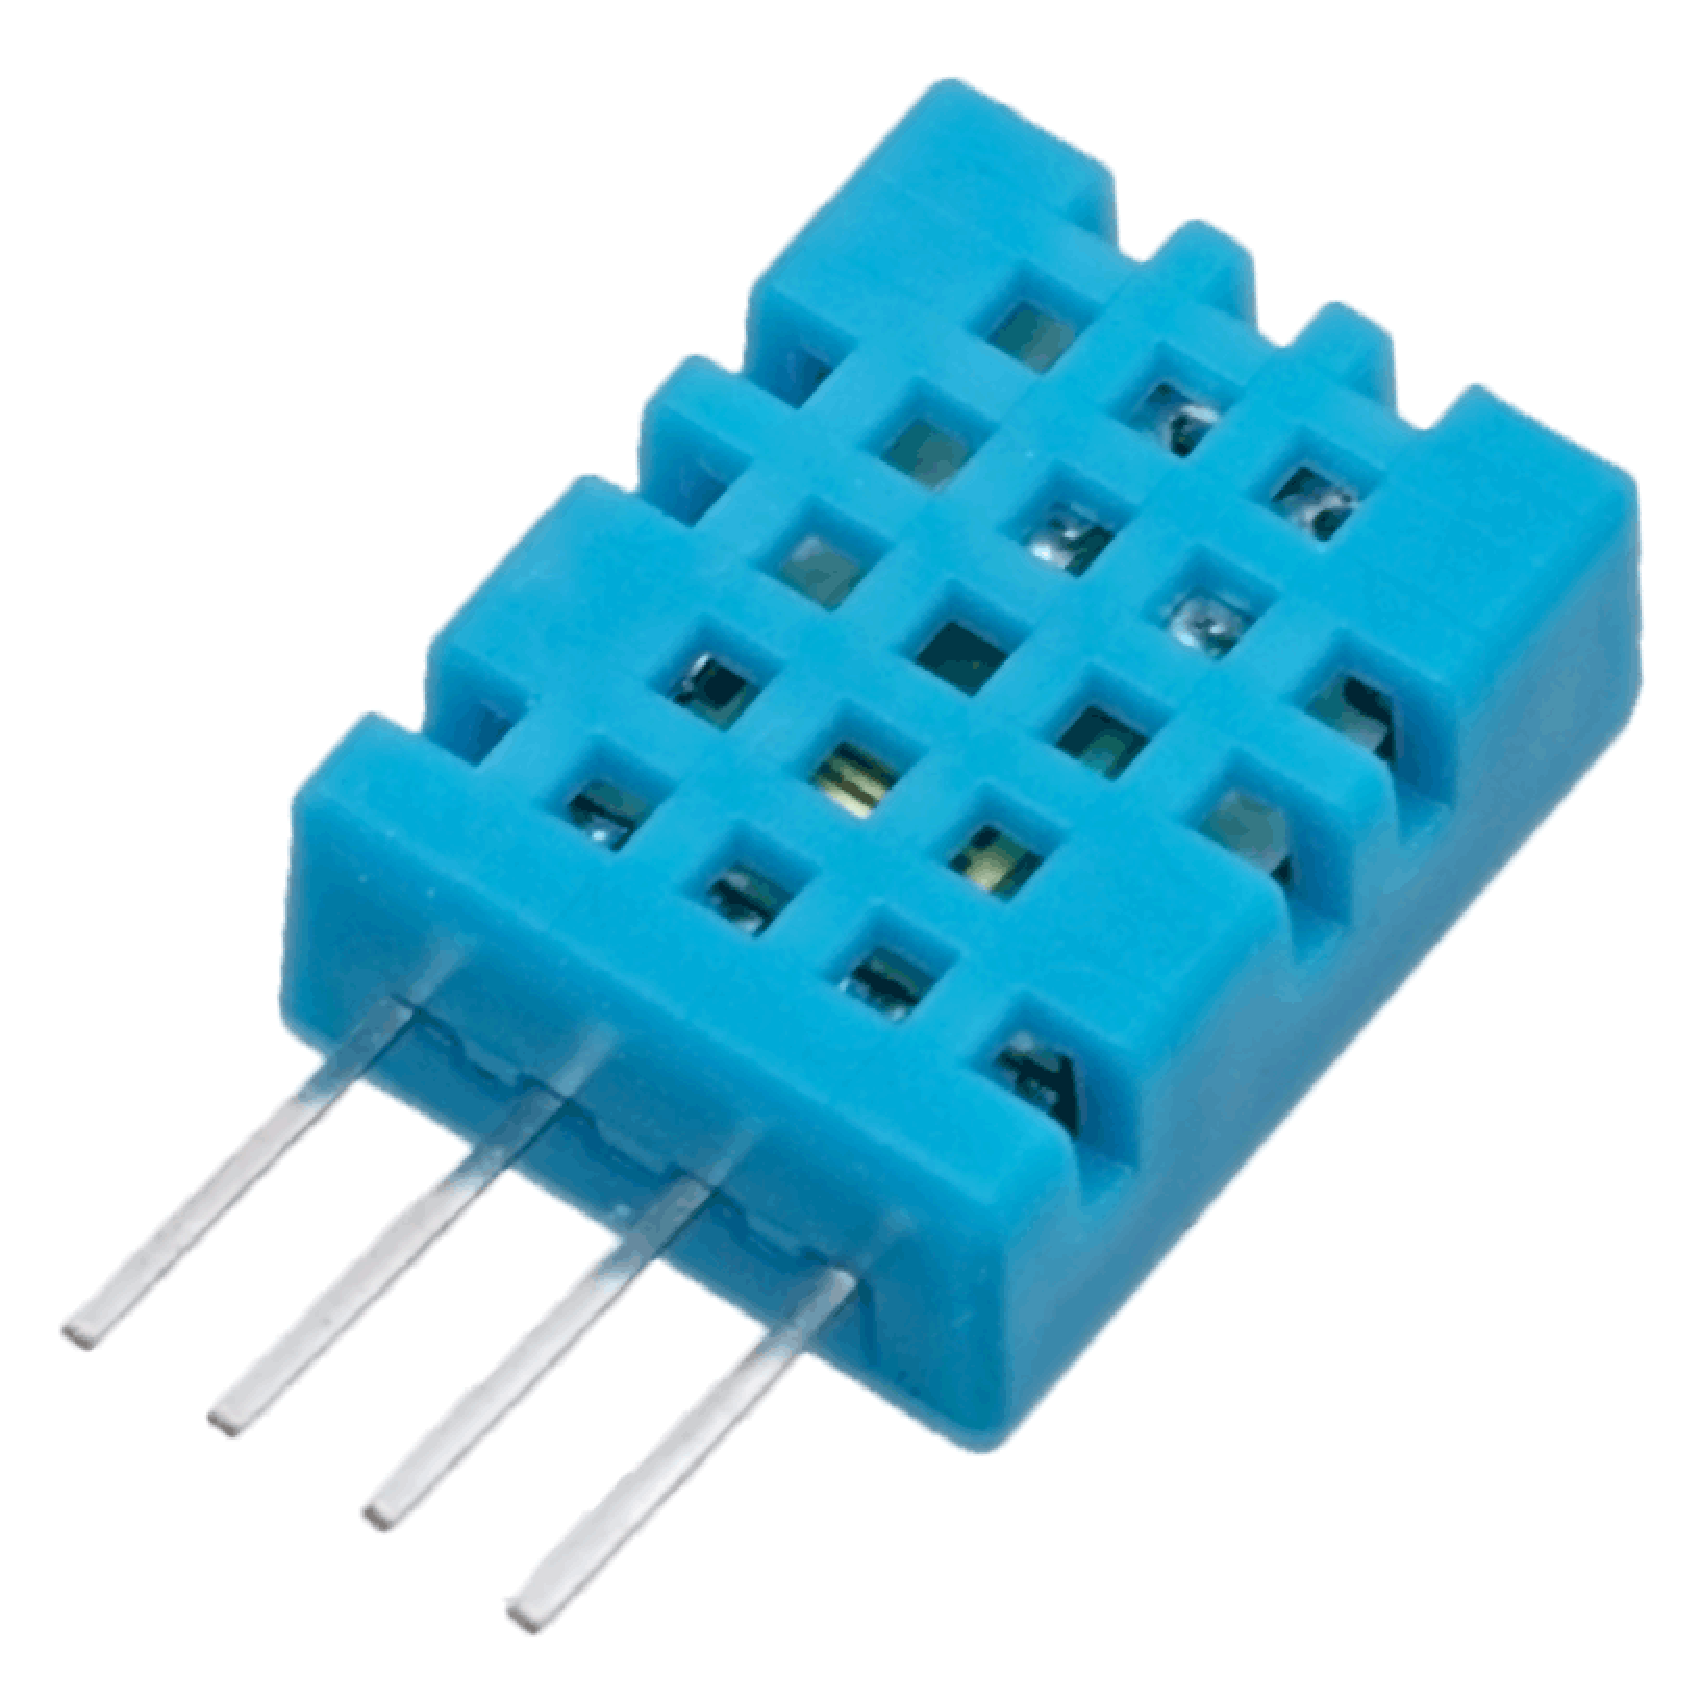
\includegraphics[keepaspectratio=true,scale=0.1]{figuras/dht-11.eps}
  \caption{\label{DHT11}Sensor de umidade relativa e temperatura do ar}
  \end{center}
  \end{figure}

  \item Sensor de Umidade do Solo

  O sensor escolhido para a medição da umidade do solo foi o HL-69,
  tanto pelo baixo custo quanto pelo simples processo de medição.
  Ele tem como princípio de medição a queda de tensão resultante da
  passagem de corrente por uma malha resistiva, que no caso seria o solo
  umedecido.

  O sensor é constituído por duas linhas de eletrodos que estão
  sobrepostas a duas placas com terminações pontiagudas para facilitar a
  penetração do sensor no solo. Uma corrente é injetada em uma das linhas
  de eletrodos e é medida a queda tensão entre as linhas, que é função da
  resistência entre os eletrodos que por sua vez é função da quantidade de
  água e minerais presentes entre os eletrodos. Quando o volume de água no
   solo entre os eletrodos é baixo, ou seja, quando o solo está seco,
   a queda de tensão será maior, e quando o solo está umedecido,
   a queda de tensão é menor.

  Devido ao seu princípio de operação, este sensor mede a quantidade de
  água no solo de forma indireta, e a calibração do sensor vai de acordo
  com o que é definido como um solo seco ou úmido em um local, e portanto
  se faz necessária a calibração do equipamento em campo junto ao
  responsável pela irrigação.

  \begin{figure}[!htbp]
  \begin{center}
  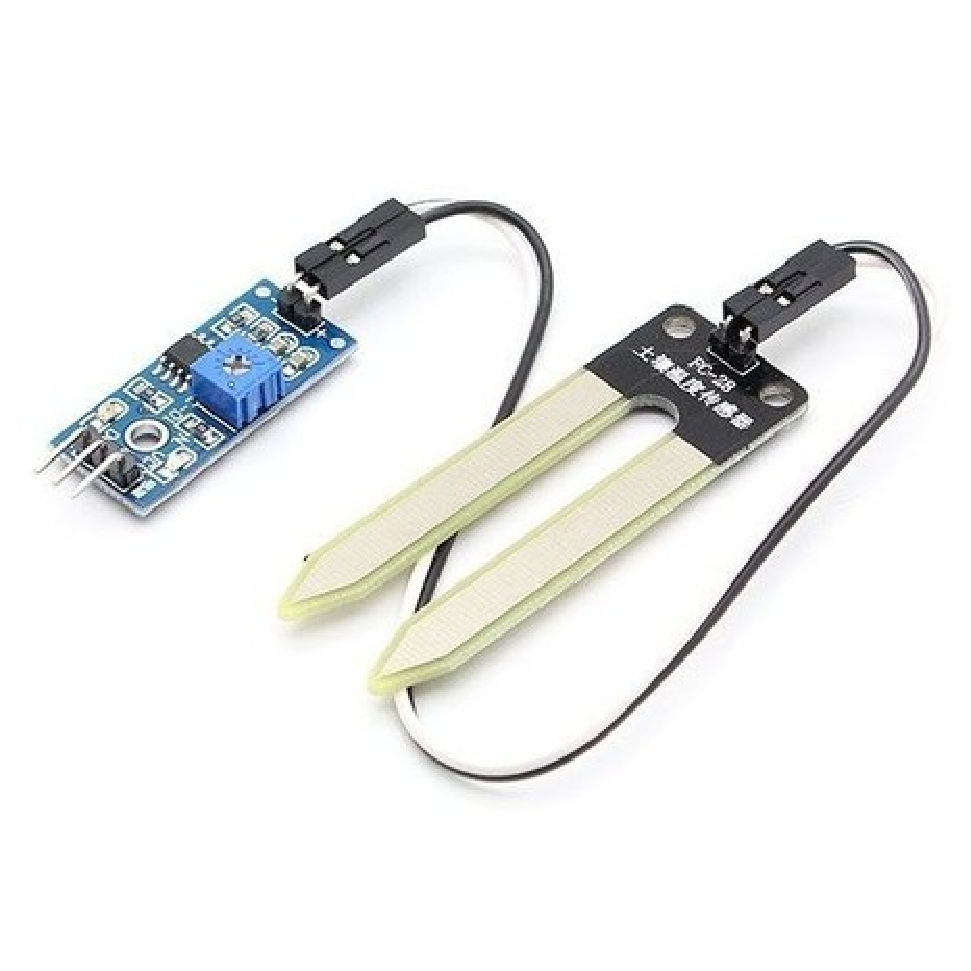
\includegraphics[keepaspectratio=true,scale=0.3]{figuras/higrometer.eps}
  \caption{\label{DHT11}Sensor de umidade do solo}
  \end{center}
  \end{figure}

  \item Modulo de Controle

  Para o controle do sistema escolheu-se a placa Arduino Mega2560.
  O Mega2560 é uma placa de microcontrolador baseado no ATmega2560 .
  Ele tem 54 pinos digitais de Entrada e saída, 16 entradas analógicas,
  4 UARTs, uma conexão USB , dentre outros. Ele contém tudo o necessário
  para dar suporte ao microcontrolador. A figura~\ref{fig:arduino} apresenta a placa
  Arduino Mega2560.

  \begin{figure}[!htbp]
  \begin{center}
  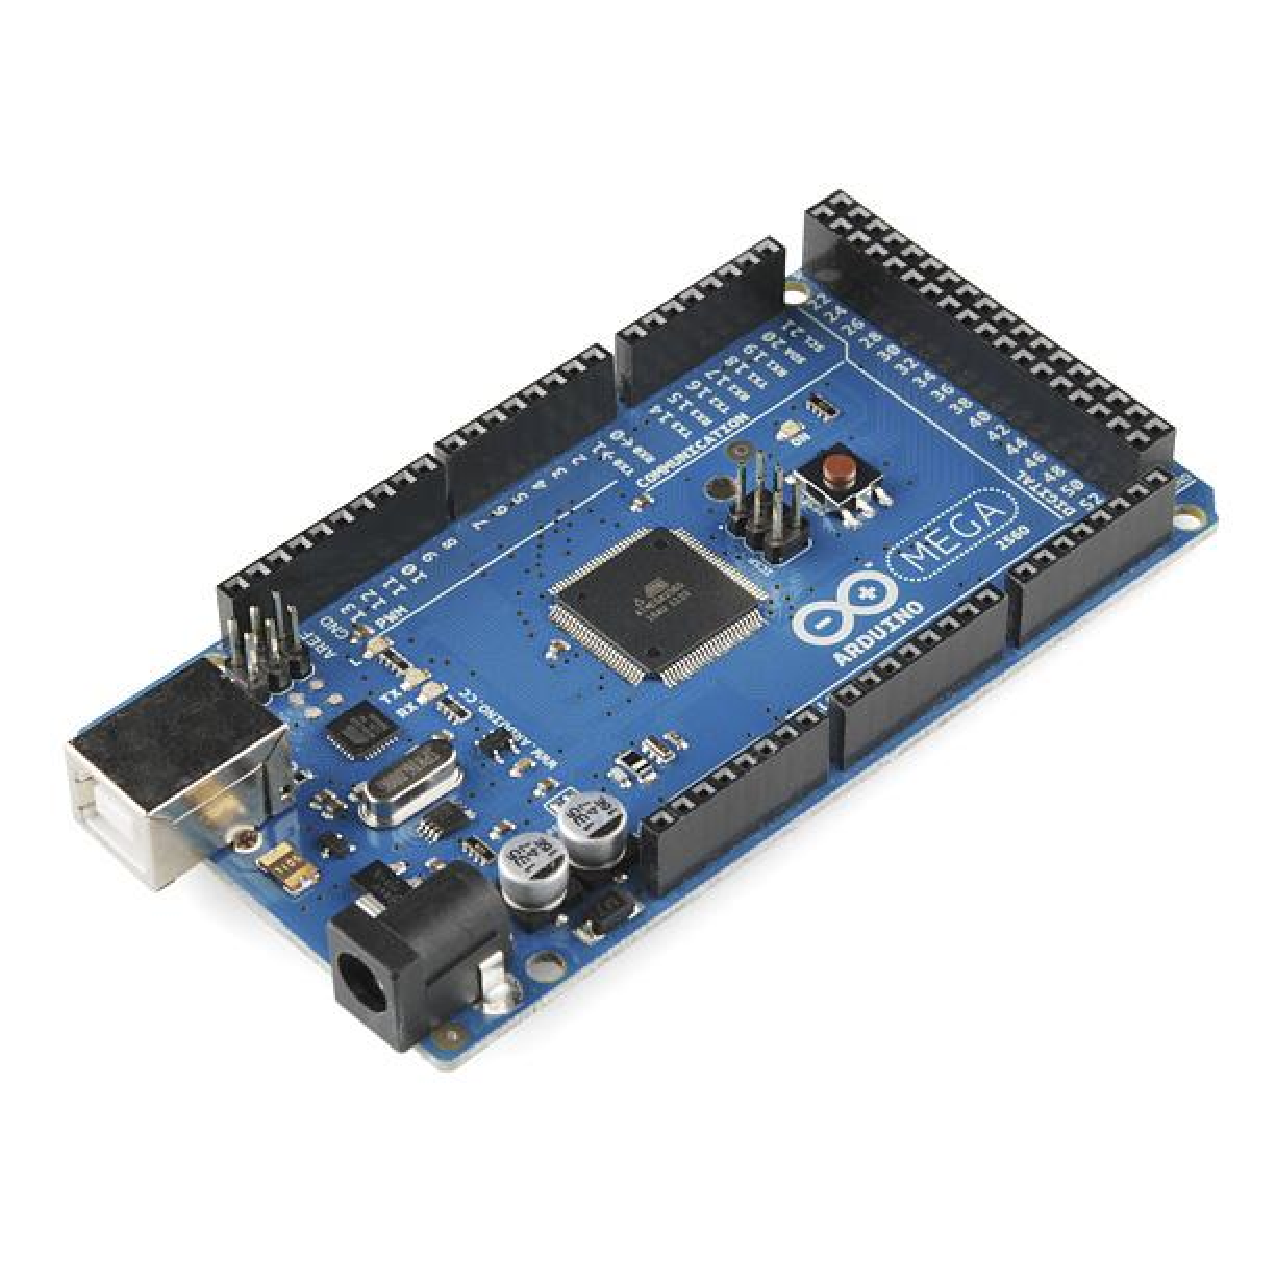
\includegraphics[width=.6\textwidth]{figuras/arduino.eps}
  \caption{\label{fig:arduino}Arduino Mega2560.}
  \end{center}
  \end{figure}

  \newpage

  A escolha da placa foi motivada por diversos fatores.
  Primeiramente, ela é capaz de realizar as demandas de controle do
  veículo, bem como possui um número de portas adequado. Além disso,
  é relativamente barata se comparada a outras plataformas de
  microcontroladores. Seu software é multiplataforma, proporcionando
  a interface com o Linux e possui um ambiente de programação simples,
  claro e bastante familiar.


  \end{itemize}
